\documentclass{article}


\usepackage{enumitem}
\usepackage[pdftex]{graphicx}
\usepackage{mathtools}


% Global '\begin{itemize}[noitemsep,topsep=0pt,parsep=0pt,partopsep=0pt]'
\setitemize{noitemsep,topsep=0pt,parsep=0pt,partopsep=0pt}


\newcommand{\argmax}[0]{\text{argmax}}
\newcommand{\para}[0]{\par\vspace{0.2cm}\noindent}
\newcommand{\define}[2]{\textbf{#1} - {#2}.  \para}


\begin{document}
\section{Stats refresher}
\define{random variable}
           {a (vector) variable whose possible values are outcomes of a random phenomenon}
\define{joint distribution}
           {n-dimensional probability distribution over n variables}
\define{marginal distribution}
           {a joint distribution over a subset of the variables; the ignored variables are summed over}
\define{information entropy}
           {the average rate at which information is produced by a stochastic source of data; or the expected information of a message}
$$ H(X) = - \sum p(x_i) \log p(x_i) \text{,  [bits, nats, bans]}$$
\para
In the case of $p(x_i) = 0$ for some $i$, the value of the corresponding summand $0 \log(0)$ is taken to be 0, which is consistent with the limit:
$$ \lim_{p \to 0+} p \log(p) = 0$$

\section{Models, Data, Learning Problems}
\subsection{Taxonomy of learning problems}
\define{instance}
           {a random variable value; a specific outcome}
\define{model}
           {a prediction mechanism; a function that maps an instance to a value of the target variable}
\define{linear model - defines a plain in n-dimensional space}
           {$y_\theta(x) = x^T \theta + \theta_0$}
\textbf{unsupervised learning}
           \begin{itemize}
                \item{find structure in data}
                \item{find attributes which describe the data well}
                \item{anomaly detection}
           \end{itemize}
\para
\define{supervised learning}
           {find the function most likely to have generated the training data}
\define{reinforcement learning}
           {control a dynamic system; the model performs experiments(exploration) while keeping the system operating nominally(exploitation)}


\subsection{Models}
\define{loss}
           {$l(y_\theta(x_i), y_i)$ - measures agreement between model predictions and true labels}
\define{empirical risk}
           {expected loss under an assumed distribution}
\define{empirical risk}
           {$\hat R(\theta) = 1/n \sum_{i=1}^n l(y_\theta(x_i), y_i)$ - expected loss over all training data $T_n$}
\define{zero-one loss}
           {$l_{0/1}$ - can be parameterised for false positive and false negative costs}
$$l_{c_FP, c_FN}(x_i) =
  \begin{cases}
    0         & \quad \mathrm{if } f(x_i) = y_i  \\
    c_{FP}    & \quad \mathrm{if } x_i = +1, y_i = -1  \\
    c_{FN}    & \quad \mathrm{if } x_i = -1, y_i = +1  \\
  \end{cases}$$


\subsection{Classification}
\define{searching for a model}
           {$\theta^* = {argmin}_\theta \sum_{i=1}^n \hat R$ - unregularized, this can have 0, 1 or many solutions}

\define{regularizer}
           {expresses prior knowledge, does not depend on the data  \\
            $l0$ - count of nonzero parameters, rarely used  \\
            $l1$ - favours sparse models  \\
            $l2$ - prevents any single parameter from becoming too important}
\para
\define{regularized empirical risk}
           {$\hat R(\theta) = \frac{1}{n} \sum_{i=1}^n l(y_\theta(x_i), y_i) + \lambda \Omega (\theta)$}

Justification for using regularizers:
\begin{itemize}
    \item{regularized loss model equivalent to MAP model in Bayesian statistics}
    \item{lower theoretical upper bond on OOB error}
    \item{select among many equally good solutions to the loss}
    \item{avoid model sensitivity to training data (stability)}
\end{itemize}
\para
\define{expected OOB loss}{
    $$R(\theta) = \sum_y \int l(y_\theta(x), y) p(x, y) dx$$
    where $p(x, y)$ - true generating joint probability distribution}

A trivial way to obtain full in-band accuracy - remember all training instances in a table.  \\
\par
Model evaluation methods:
\begin{itemize}
    \item{training and test datasets}
    \item{N-fold cross validation.}
\end{itemize}


\section{Problem Analysis and Data Prepossessing}
\subsection{types of problems}
Data availability challenges
\begin{itemize}
    \item{number of data: too few? too many for a single CPU main memory?}
    \item{number of attributes: too few? too many? sparse?}
    \item{quality: missing values? erroneous values? measurement error?}
\end{itemize}
\par
Data integration challenges
\begin{itemize}
    \item{format and measurement units}
    \item{identify same/similar attributes in the different databases}
    \item{conflicts}
    \item{redundancy}
\end{itemize}


\subsection{Representation properties of data}
\begin{itemize}
    \item{number of classes - 2 vs 50 000}
    \item{class ratio - balanced vs rare classes}
    \item{$p_{train}(x) = p_{application}(x)$ - same generating process}
    \item{$p_{train}(y|x) = p_{application}(y|x)$ - same labelling process}
    \item{is the training sample representative of class frequency? else we are operating under 'covariate shift'}
    \item{data getting old}
    \item{separate data sources with different quality measures}
\end{itemize}
\para
\define{data warehouse}
           {a database which has been optimised for analytic processes, instead of for transactional processes}


\subsection{Encoding}
Linear models expect numeric inputs.
\para
Encode categorical variables one-hot, otherwise we are making an assumption of orderliness of the values.
\para
\define{TF representation}
           {term frequency - a set of \{word:count\},
            possibly trimmed below e.g. f=3}
\define{TFIDF representation}
           {terms that occur often (or, and, is) carry little semantic power - assign lower weights}
            $$\text{inverse document frequency}
                = \log \frac{\text{num documents}}{\text{num documents that contain the term}}
                = \log \frac{N}{n_T}$$

$$
TFIDF(x) = \frac{1}{|x|}
 \begin{pmatrix}
  TF({term}_1) * IDF({term}_1)  \\
  \vdots  \\
  TF({term}_n) * IDF({term}_n)  \\
 \end{pmatrix}
$$

where $|d|$ - count of words in this text of the corpus
\para
To preserve structure information in text, n-grams are used.
We have to introduce 1 new attribute per n-tuple.
Fortunately results are sparse.


\subsection{Feature normalisation}
Non-normalised data results in unbound weights.
The regularizer doesn't know if a weight is large because the feature is important, or because of scaling.
\begin{itemize}
    \item{min/max}
    \item{z-score}
    \item{decimal scaling}
    \item{log scaling}
\end{itemize}


\subsection{Introducing new features}
Hand-crafting new features as function of old features, which is outside the model's search space.
E.g. polynomial kernels consider all polynomials of the input variables, but linear models don't.


\subsection{Handling missing, erroneous values}
\begin{itemize}
    \item{delete instances (if few) or attributes(if almost always missing)}
    \item{add a value 'missing' OR introduce a binary attribute val\_missing}
    \item{interpolate - class specific mean/median; or infer most likely value}
\end{itemize}
\para
Erroneous values identification is performed by either binning or clustering.
Small resulting sets are suspect outliers.
\par
Some classes might exhibit missing values more often then others e.g. user provided credit rating.


\subsection{Feature selection}
\begin{itemize}
    \item{PCA}
    \item{foreword/backward elimination - try model with 1 attribute, test, train with 2 attributes, test, if better continue}
    \item{for a linear model - train a model on all attributes, delete attributes with smallest weights, retrain}
\end{itemize}


\section{Decision trees}
\subsection{Introduction}
\define{test node}
           {tests one attribute}
\define{edge}
           {one specific outcome of the testing}
\define{terminal node}
           {contains a prediction}

Advantages:
\begin{itemize}
    \item{understandable to a domain expert}
    \item{fast predictions}
    \item{nonlinear model - thus can represent nonlinear functions}
    \item{provides reasoning behind the prediction}
    \item{can be expressed as a logical rule by walking the branch from root to leaf}
\end{itemize}

\define{classification model}
           {a mapping from vectors X to a categorical variable, called labels, classes}
\define{regression model}
           {a mapping from vectors X to real numbers}

\begin{verbatim}
Learning decision trees
    Why prefer smaller trees
        easy to interpret
        more training instances per leaf node
So - smallest decision tree, that is consistent with the training data.
\end{verbatim}


\subsection{Classification with categorical features: ID3}
A greedy algorithm, which finds a small tree.
polynomial complexity($n^{const}$) in the number of attributes
\begin{verbatim}
ID3(L):
if all data in L has same class y, then return leaf node with class y else
1. choose the attribute xj with the most homogeneous class distribution (max(GR_L(x_j))) 
2. split L into one set per value of the attribute
3. return a test node with xj and the subsets as children
\end{verbatim}

\define{n-optimal code}
           {assign short code words to common events}

\define{information of a message}
           {$-\log_2 p(y=v)$, where $v$ - this specific message value}

\define{expected information of a message(entropy)}
           {$$ H(y) = -\sum_{v=1}^k p(y=v) \log_2 p(y=v) $$}

\define{empirical entropy $H_L$}
           {learned on sample L}

\define{entropy of class labels}
           {$H_L(y) = - \sum p(y_i) \log_2 p(y_i)$}

\define{conditional entropy}
           {$H_L(y|x=n) = -p_{x=n} \log p_{x=n} +
                          -p_{x \neq n} \log p_{x \neq n}$}

\define{information gain}
           {reduction of entropy by splitting the data along an attribute}
$$ G_L(x_j) = H_L(y) - \sum_{v=1}^k p_L(x_j=v) H_L(y|x_j=v) $$

\define{entropy of an ATTRIBUTE}
           {$$ H_L(x_j) = - \sum_{v=1}^k p_L(xj=v) logp_L(x_j=v) $$}

\begin{verbatim}
IG is biased towards many-valued attributes 
e.g. matriculation number as predictor of exam performance
it does not generalise well
\end{verbatim}

\define{information gain ratio}
           {weight IG by the entropy of the attribute values}
$$ GR_L(hj) = \frac{G_(x_j)}{H_L(x_j)} $$


\subsection{Classification with continuous features: C4.5}
We now label test nodes with \{attribute; threshold value\}.

$$ G_L(x_j \leq v) = H_L(y) - p_L(x_j \leq v) H_L(y|x_j \leq v) - p_L(x_j > v) H_L(y|x_j > v)$$

\begin{verbatim}
if all data has the same class OR is identical, predict the majority class
else
    for categorical variables, calculate $GR_L(x_j)$
        for each continuous attribute
            for each value v_i it takes
                calculate $GR_L(x_j \leq v_i)$
    select a split
        if discrete, split as ID3 and do recursion
        if continuous, we create a binary node $x_j \leq v$ and do recursion
\end{verbatim}

Leaf nodes trained on very few training instances are not to be trusted.

\define{pruning with support threshold}
           {removing of leaf nodes, whose support is less than a threshold}

\begin{verbatim}
how it's done:
    remove the leaf node
    replace it's parent test node with a leaf note
    it contains the majority class of both removed leaf nodes
\end{verbatim}

\define{reduced error pruning}
           {train/test split, remove 1 leaf node from a trained tree, if loss is reduced, keep the change}


\subsection{CART}
Regression trees
\define{Mean squared error}
           {$MSE = \frac{1}{n} \sum_{i=1}^n (f(x_i) - y_i)^2$}

Notice that
$$ var(X) = \frac{1}{n} \sum_{i=1}^n (\overline y - y_i)^2$$
In our leaf nodes, we must put concrete numeric values.
So we can reduce the expected error by grouping similar values and assigning their mean as leaf value. 

Splitting criterion: variance reduction
$$ R_L[x_j \leq v] = var(L) - \frac{n_{[x_j \leq v]}}{n} var(L_{[x_j \leq v]})
                            - \frac{n_{[x_j > v]}}{n} var(L_{[x_j > v]})$$
,where L - labels
n - total number of instances

\define{stopping criterion}
           {$n * var(L) \leq \tau$ - if true, do not create a test node, but a leaf node}

\begin{verbatim}
if stopping criterion is satisfied create a leaf node else
for discrete attributes calculate R_L(x_j)
for continuous attributes iterate over all v and again determine R_L(x_j, v_i)
create a split at highest variance reduction
\end{verbatim}

\define{model tree}
           {instead of putting a number in the leaf node, put a local regression mode, learned only on the datapoints which constitute the leaf}

Linear regression model
$$ f(x) = \theta^T x + \theta_0  $$

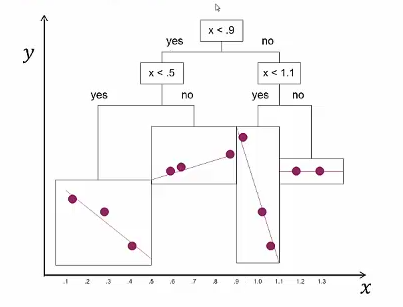
\includegraphics[height=0.4\textheight]{model_tree}


\subsection{Bagging(ensemble learning)}
Motivation:
Let us have 3 classifiers, each with error probability of 0.1.
Let $f(x)$ be the majority vote among $f_i(x)$
$$ f(x) = \argmax|y \{i: f_i(x) = y $$
Error probability of the ensemble?
    if models are the same - 0.1
    if totally unrelated - $R \leq 3 * 0.1^3 = 0.03$

All in all ensemble learning is great if:
    each model's error probability is less than 0.5
    the models need to be sufficiently correlated

Ensemble models differ in how do they obtain uncorrelated models on the dataset.

\define{bagging}
           {draw random subsets of the training instances for each model}

\define{random forest}
           {draw random subsets of training data + random subsets of features}

\define{boosting}
           {increase weight of misclassified instances}

\define{bootstrapping}
           {draw instances uniformly with replacement}

If we bootstrap n samples from n-sample long database, about 60\% of the instances will be included.

\define{bagging}
           {an ensemble learning method - aggregation of bootstrapping}
bootstrap k models
return one model
    for classification - majority vote
    for regression - average
Problems: different data, but same generating distribution - models not independent
  
\define{random forest}
           {like bagging, but also randomly draw m(hyperparameter) attributes}  
decision trees have maximum dept
no pruning applied - the voting is a form of regularization

How many trees(1000):
    the more the better
    computational power
    dataset size - we start drawing identical random subsets

\subsection{Random forests}

\subsection{Viola-Jones}
Face detection
24x24 pixels
uses HAAR features - 
    efficient to calculate via an integral image (computed in a single pass)
$$ I_{int}(x, y) = \sum_{x` \leq x, y' \leq y} I(x`, y`) $$

\define{decision stump}
           {decision tree of depth 1}

\begin{verbatim}
for all available haar features (type, position, size, polarity, threshold)
calculate split criterion(reduction or error rate??)
create a test node with a Haar feature (decision stump)
apply AdaBoost to collect stump decisions
reduce threshold until we miss no faces
go to next layer with only the approved images

\end{verbatim}

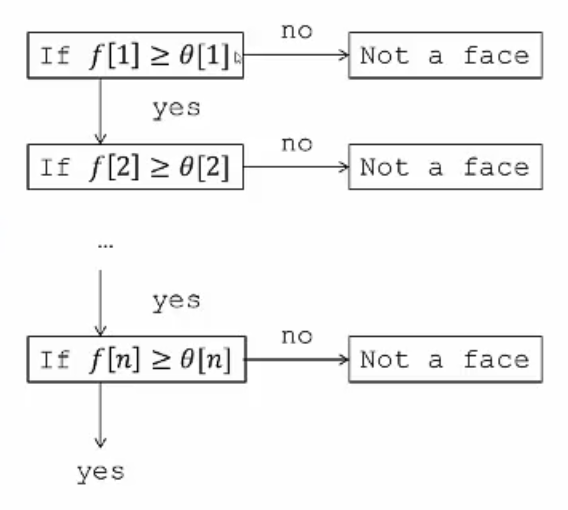
\includegraphics[height=0.5\textwidth]{haar}



\end{document}
